\documentclass[tikz,border=10pt]{standalone}
\usetikzlibrary{calc, arrows.meta, positioning, backgrounds}

\begin{document}

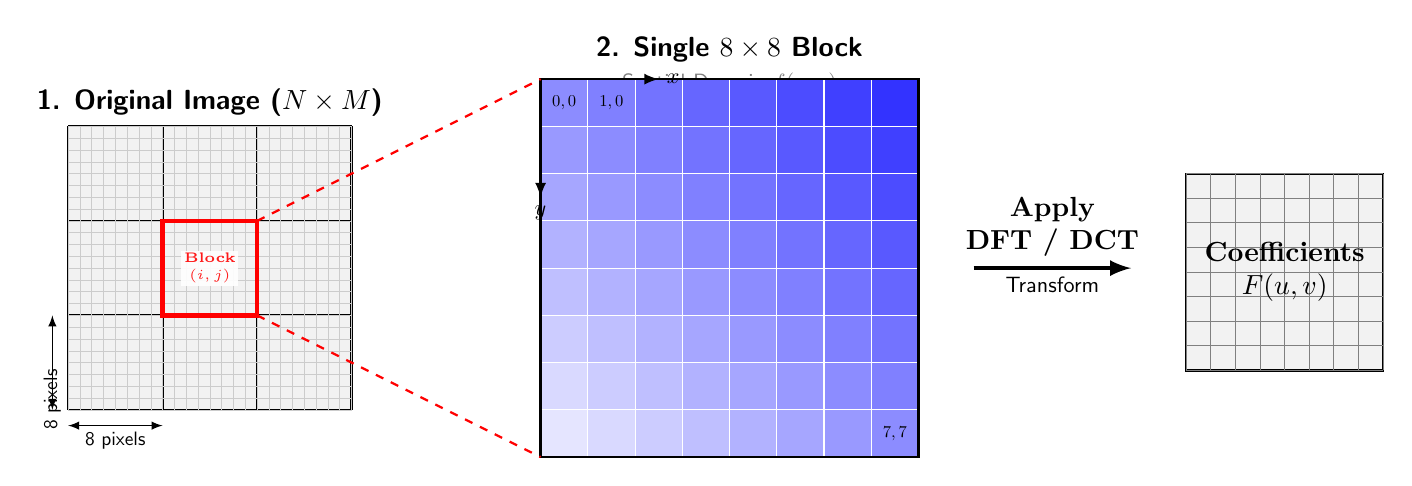
\begin{tikzpicture}[>=latex, font=\sffamily]

% --- DEFINITIONS ---
\def\pixelSize{0.15}    % Size of pixels in the main image
\def\blockSize{1.2}     % 8 * 0.15 = 1.2
\def\zoomPixelSize{0.6} % Size of pixels in the zoomed block
\def\zoomBlockSize{4.8} % 8 * 0.6 = 4.8

% --- 1. MAIN IMAGE (Left Side) ---
\node[above] at (1.8, 3.6) {\textbf{1. Original Image ($N \times M$)}};

% Draw "pixels" (simulated with a gray background)
\fill[gray!10] (0,0) rectangle (3.6, 3.6);

% Draw the 8x8 BLOCK GRID (Thick lines)
% We draw a 3x3 grid of blocks (representing a 24x24 pixel image area)
\draw[step=\blockSize, black, thick] (0,0) grid (3.6, 3.6);

% Draw the PIXEL GRID (Thin lines) inside the blocks
\draw[step=\pixelSize, gray!40, very thin] (0,0) grid (3.6, 3.6);

% Highlight the center block (Target for extraction)
\draw[red, ultra thick] (\blockSize, \blockSize) rectangle (2*\blockSize, 2*\blockSize);
\node[red, font=\bfseries\tiny, align=center, fill=white, inner sep=1pt, opacity=0.9] 
    at (1.5*\blockSize, 1.5*\blockSize) {Block\\$(i,j)$};

% Annotations for the main image
\draw[<->] (0, -0.2) -- (\blockSize, -0.2) node[midway, below, scale=0.7] {8 pixels};
\draw[<->] (-0.2, 0) -- (-0.2, \blockSize) node[midway, left, scale=0.7, rotate=90] {8 pixels};


% --- 2. ZOOMED 8x8 BLOCK (Center) ---
\begin{scope}[shift={(6, -0.6)}]
    \node[above] at (2.4, 4.9) {\textbf{2. Single $8 \times 8$ Block}};
    \node[above, gray, scale=0.8] at (2.4, 4.5) {Spatial Domain $f(x,y)$};

    % Draw individual pixels of the 8x8 block
    \foreach \x in {0,...,7} {
        \foreach \y in {0,...,7} {
            % Simulate data values with varying shades of blue
            \pgfmathsetmacro{\shade}{10 + (\x+\y)*5}
            \fill[blue!\shade!white] (\x*\zoomPixelSize, \y*\zoomPixelSize) rectangle ++(\zoomPixelSize, \zoomPixelSize);
            % Draw pixel borders
            \draw[white, thin] (\x*\zoomPixelSize, \y*\zoomPixelSize) rectangle ++(\zoomPixelSize, \zoomPixelSize);
        }
    }
    % Border around the whole zoomed block
    \draw[black, thick] (0,0) rectangle (\zoomBlockSize, \zoomBlockSize);

    % Coordinate labels (x,y)
    \node[scale=0.6] at (0.5*\zoomPixelSize, 7.5*\zoomPixelSize) {$0,0$};
    \node[scale=0.6] at (1.5*\zoomPixelSize, 7.5*\zoomPixelSize) {$1,0$};
    \node[scale=0.6] at (7.5*\zoomPixelSize, 0.5*\zoomPixelSize) {$7,7$};
    
    % Axes
    \draw[->, thick] (0, \zoomBlockSize) -- (1.5, \zoomBlockSize) node[right, scale=0.8] {$x$};
    \draw[->, thick] (0, \zoomBlockSize) -- (0, \zoomBlockSize-1.5) node[below, scale=0.8] {$y$};
\end{scope}


% --- 3. CONNECTION LINES (Zoom Effect) ---
% Connect the corners of the highlighted red block to the zoomed block
\draw[red, dashed, thick] (2*\blockSize, 2*\blockSize) -- (6, \zoomBlockSize-0.6); % Top right to Top Left
\draw[red, dashed, thick] (2*\blockSize, \blockSize) -- (6, -0.6);   % Bottom right to Bottom Left


% --- 4. DFT APPLICATION ARROW ---
\draw[->, ultra thick, align=center] (11.5, 1.8) -- (13.5, 1.8) 
    node[midway, above, font=\bfseries] {Apply\\DFT / DCT}
    node[midway, below, scale=0.8] {Transform};

% --- 5. FREQUENCY DOMAIN HINT (Right Side) ---
\begin{scope}[shift={(14.2, 0.5)}]
    \draw[fill=gray!10, thick] (0,0) rectangle (2.5, 2.5);
    \draw[step=0.3125, gray] (0,0) grid (2.5, 2.5);
    \node[align=center, font=\bfseries] at (1.25, 1.25) {Coefficients\\$F(u,v)$};
\end{scope}

\end{tikzpicture}

\end{document}